\pagestyle{kalinka}
\label{kalinka}

\begin{textblock*}{5.625in}(0pt,0pt)%
\vspace*{-2.35cm}
\hspace*{-1.65cm}\includegraphics*[width=160mm]{./imgs/KALINKA.png}
\end{textblock*}

\pagebreak %A CIDADE ENE

\hspace{.5cm}

\begin{center}
\hspace*{.5cm}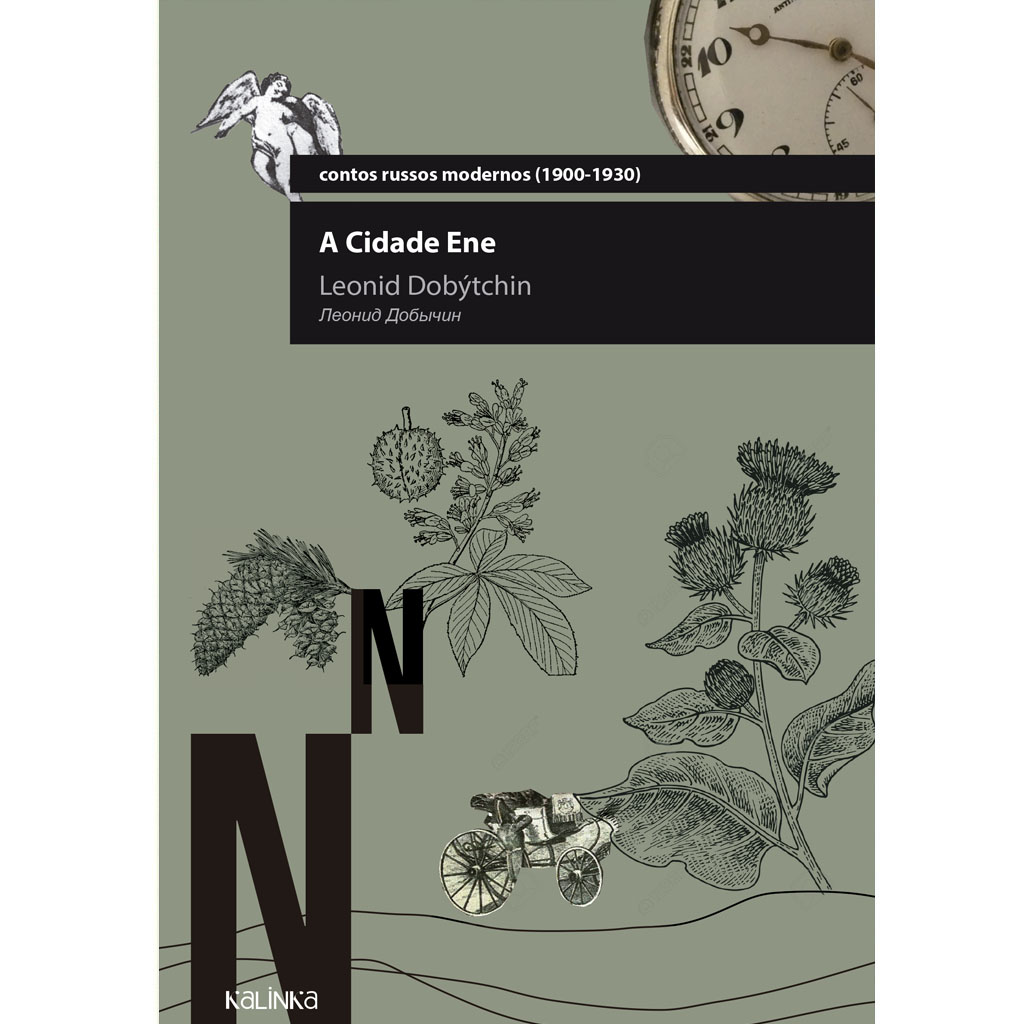
\includegraphics[width=92mm]{./grid/cidaden.jpg}
\end{center}

\hspace*{-7cm}\hrulefill\hspace*{-7cm}

\medskip

\noindent{}{\slsc{A Cidade Ene}} é uma narrativa do ponto de vista de uma criança do começo do século \scalebox{.8}{XX}. Desvelam"-se reminiscências de uma Rússia pré"-revolucionária e sua burguesia decadente e provinciana. Na fictícia cidade Ene --- em homenagem à cidade de {\slsc{Almas mortas}} de Gógol --- são percebidas fortes características de Daugavpils, onde o autor Leonid Dobýtchin viveu boa parte da vida. Embora seja também um lugar simbólico, um todo"-lugar, representando o conjunto dos ambientes urbanos russos: ao buscar continuidades, questiona"-se a real profundidade produzida pela Revolução  no homem e na sociedade.

Com uma das histórias mais trágicas da história literária russa, já repleta de infortúnios, o autor não teve sua própria mesa para escrever até os 40 anos, quando recebeu da União dos Escritores Soviéticos um quarto num apartamento comunal em São Petersburgo, dois anos antes de falecer em presumido suicídio. Perseguido pela máquina de censura stalinista, foi taxado como “formalista”. Ele se defendeu das acusações e desapareceu no dia seguinte, nunca mais ninguém o viu.

\vfill

\hspace*{-.4cm}\begin{minipage}[c]{.5\linewidth}
\small{
{\Formular{\textbf{
\hspace*{-.1cm}Título: A Cidade Ene\\
Autor: Leonid Dobýtchin\\ 
ISBN: 978-65-8686-200-3\\
Páginas: 142\\
Formato: 14x21cm\\
Preço: R\$ 42,90\\
Editora: Kalinka\\
Disponibilidade: 17/07/2020
}}}}
\end{minipage}


\pagebreak

\begin{changemargin}
\hspace{.5cm}
\vspace*{1cm}
\enlargethispage{-\baselineskip}

\noindent{}{\LARGE{Porta de entrada da obra de Dostoievski, `Bobók' ganha nova tradução\\\noindent{}{\large\slsc{Livro é um microcosmo do trabalho do autor russo}}}}

\bigskip

\hfill{}\scalebox{.8}{GUTEMBERG MEDEIROS}

\bigskip

“Todos nós saímos do {\slsc{Capote}} de Gogol”. Esta frase de Fiodor Dostoievski (1821--1881) dirigida aos seus colegas escritores marcou de modo decisivo a literatura russa. Aqui se resumem várias qualidades herdadas de Gogol, especialmente o mundo do riso imprimindo pesada crítica social. Um exemplo dos mais felizes dessas marcas está na edição de {\slsc{Bobók \& Meia Carta de um Sujeito}} (Editora Kalinka), em tradução direta assinada por Mossei e Daniela Moutian. 

Ambos os textos curtos misturam jornalismo e literatura com os mais diversos matizes de humor. Um texto dialoga diretamente em ironia com o outro, tendo sido publicados no mesmo ano, 1873, e local, o semanário conservador {\slsc{Gradjanin}} (O Cidadão). {\slsc{Bobók}}, publicado anteriormente pela Editora 34 com tradução de Paulo Bezerra, é reconhecido pela crítica como uma das peças máximas de Dostoiévski. 

{\slsc{Bobók}} pode ser visto como uma das melhores portas para entrar no mundo de Dostoievski. Segundo o pensador russo Mikhail Bakhtin, é quase um “microcosmo” de toda a sua obra. Muitas das ideias, temas e imagens estão aqui presentes de forma incisiva e explícita: a questão da existência de Deus e se “tudo é permitido” – verdadeira matriz ética e estética da condição humana –, a verdade e a mentira, a volúpia e a consciência sempre beirando a loucura. “Todos esses temas e ideias foram inseridos, de forma condensada e clara.” Além da carpintaria de texto peculiar. 

A exemplo de {\slsc{Humilhados e Ofendidos}}, o conto já inicia em tom de autoficção do autor em relação à crítica de seu tempo. O enredo é sobre o escritor Ivan Ivanovitch, sem lugar no jornalismo e no mercado editorial. Vive de expedientes pequenos. “O que mais faço é traduzir do francês para livreiros. Escrevo anúncios para comerciantes (\ldots{}) Por encomenda de um livreiro, redigi {\slsc{A Arte de Satisfazer as Mulheres}}.” O personagem alega ser visto como louco por colegas escritores e jornalistas. Trata"-se de resposta sarcástica às violentas críticas ao romance {\slsc{Os Demônios}} (1872) ao trabalhar o terrorismo de esquerda da época. Levantando"-se até suspeitas sobre a sanidade mental do autor.

Ivan acompanha um enterro e fica a pensar sobre a sua vida neste cenário. Ele cai no sono e acorda ouvindo vozes, apesar de estar só. Até perceber que as vozes emergem dos túmulos, são os mortos a falar e até a jogar cartas entre eles. Bobók é tanto onomatopeia sem sentido e também significa “fava” em russo, um balbuciar que ecoa em sua cabeça antes das vozes dos mortos. 

A partir da sucessão de diálogos, constrói"-se a reflexão de quem realmente está morto ou vivo, os que andam sobre a terra ou nela enterrados? Além disso, as máscaras sociais são abandonadas e os enterrados falam de si e de outros com absoluta sinceridade, a revelar segredos até sórdidos. Impossível não lembrar de {\slsc{Memórias Póstumas de Brás Cubas}} de Machado de Assis, que segue o mesmo diapasão. 

A acidez da crítica social de Dostoievski, por exemplo, emerge quando um morto se dirige a outro chamando"-o de conde. Este responde ser, na verdade, barão. “Somos pequenos barões sarnentos, oriundos de lacaios, mas, não sei por que, não dou a mínima. Sou apenas um patife da pseudoalta sociedade”. Em outro momento, outro morto fala abertamente de colega que amealhou fortuna na corrupção, ao roubar 400 milhões dos cofres públicos, destinados a viúvas e órfãos. Mas foi velado como reserva moral da nação. 

No texto, Ivan declara que “para compor uma opinião, é necessário escutar em todos os lugares, não apenas em um”, ou seja, saber o que menos privilegiados em vida têm a dizer. Para quê? Para tentar publicar no jornal {\slsc{O Cidadão}}, no qual {\slsc{Bobók}} foi realmente impresso. 

{\slsc{Meia Carta de um Sujeito}} é uma espécie de processo metajornalístico. É a história de um editor – cargo que Dostoievski ocupava no jornal – que recebe uma carta de leitor. O texto já inicia informando que é o mesmo sujeito que enviou outro texto sobre “tumulozinhos”, ou seja, o autor de {\slsc{Bobók}}, e avisa que só vai publicar metade do que foi enviado. Mais uma vez, o efeito de mascaramento e riso gogoliano. O editor justifica a tesourada. “A primeira metade da carta, definitivamente, é impublicável. São apenas investidas pessoais e ofensas contra quase todas as editoras de São Petersburgo e Moscou, e aqui ultrapassou todos os limites”. Após as considerações do editor, este reproduz a carta na íntegra e discute com a mesma. Dostoievski, mais uma vez, alimenta controvérsias com outros veículos e jornalistas de seu tempo, devidamente explicadas em ricas notas de rodapé de página preparadas pelos tradutores. 

Dostoievski foi um dos mais importantes e populares jornalistas em seu tempo, tendo dedicado boa parte de sua vida ao jornalismo ao travar extensas polêmicas, consumando reflexões sobre as relações entre ser humano, contexto histórico e memória. Uma das principais características do {\slsc{Diário de um Escritor}}, origem desses dois contos, é ser um produto construtor de memória, ou “a palavra retirada da vida” (em que local começa a citação?), conforme a definição do filósofo Mikhail Bakhtin.\footnote{Publicado originalmente em {\slsc{O Estado de S. Paulo}}, em 22 de setembro de 2018.}

\pagebreak
\end{changemargin}
\pagebreak

\pagebreak
\pagestyle{kalinkacat}

\begin{multicols}{2}
\begin{enumerate}
\item O compromisso, {\Formular{\textbf{Serguei Dovlátov}}}
\item Aulas de literatura russa, {\Formular{\textbf{Aurora Fornoni Bernardini}}}
\item O Elefante, {\Formular{\textbf{Aleksandr Kuprin}}}
\item A Velha, {\Formular{\textbf{Daniil Kharms}}}
\item Bobok E Meia Carta De Um Sujeito, {\Formular{\textbf{Fiódor Dostoiévski}}}
\item Parque cultural, {\Formular{\textbf{Serguei Dovlátov}}}
\item O diabo mesquinho, {\Formular{\textbf{Fiódor Sologub}}}
\item Tarakã, o bigodudo, {\Formular{\textbf{Kornei Tchukóvski}}}
\item Salmo, {\Formular{\textbf{Friedrich Gorenstein}}}
\item O Oficio, {\Formular{\textbf{Serguei Dovlátov}}}
\item Luminescência, {\Formular{\textbf{Viatchesláv Kupriyánov}}}
\item Poesia russa, {\Formular{\textbf{Vários}}}
\item Encontros com Liz e outras histórias, {\Formular{\textbf{Leonid Dobýtchin}}}
\item Os sonhos teus vão acabar contigo, {\Formular{\textbf{Daniil Kharms}}}
\end{enumerate}
\end{multicols}

\pagebreak




%\hspace{.5cm}
%
%\begin{center}
%\hspace*{-1cm}\raisebox{5.5cm}{\rotatebox[origin=t]{90}{\Formular{\textbf{Lançamento}}}}
%\hspace{1cm}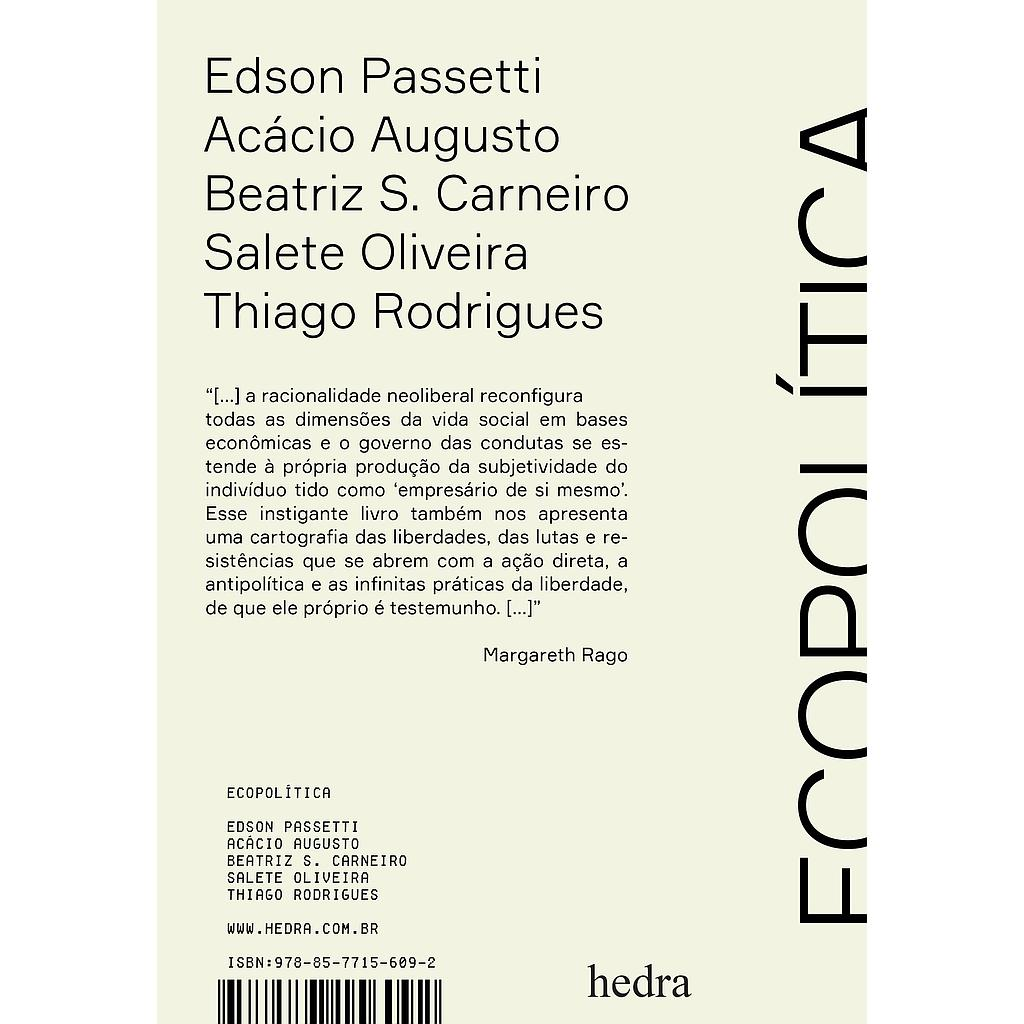
\includegraphics[width=70mm]{eco.jpeg}
%\end{center}
%
%\hspace*{-2cm}\_\_\_\_\_\_\_\_\_\_\_\_\_\_\_\_\_\_\_\_\_\_\_\_\_\_\_\_\_\_\_\_\_\_\_\_\_\_\%_\_\_\_\_\_\_\_\_\_\_\_\_\_\_\_\_\_\_\_\_\_\_\_\_\_\_\_\_\_\_\_\_\_\_\_
%
%\medskip
%
%\noindent{}Lorem ipsum dolor sit amet, consectetur adipiscing elit.
%Donec sodales tortor a purus accumsan, ut ultricies purus
%maximus. Aliquam bibendum consequat mi, sed commo-
%do velit pellentesque id. Vivamus ultricies ligula in semper
%sagittis. Donec mollis odio in lectus tristique, sed convallis
%est interdum. Cras eget sem condimentum, pretium purus
%eu, auctor.
%
%\hspace{.5cm}
%
%\hspace*{-.4cm}\begin{minipage}[c]{0.45\linewidth}
%\small{
%{\Formular{\textbf{
%\hspace*{-.1cm}Título: Ecopolítica\\
%Autor: Edson Passetti\\ 
%Editora: Hedra\\
%Páginas: 476\\
%Formato: 23x16cm\\
%Preço: R\$ 79,90\\
%}}}}
%\end{minipage}
%\begin{minipage}[c]{0.50\linewidth}
%\small{Lorem ipsum dolor sit amet, consectetur adipiscing elit. Donec sodales tortor a purus accumsan, ut ultricies. Lorem ipsum dolor sit amet, %consectetur adipiscing elit. Lorem ipsum dolor sit amet. Lorem ipsum dolor sit amet.} 
%\end{minipage}
%
%\pagebreak
%
%\hspace{.5cm}
%
%\begin{center}
%\hspace*{-.5cm}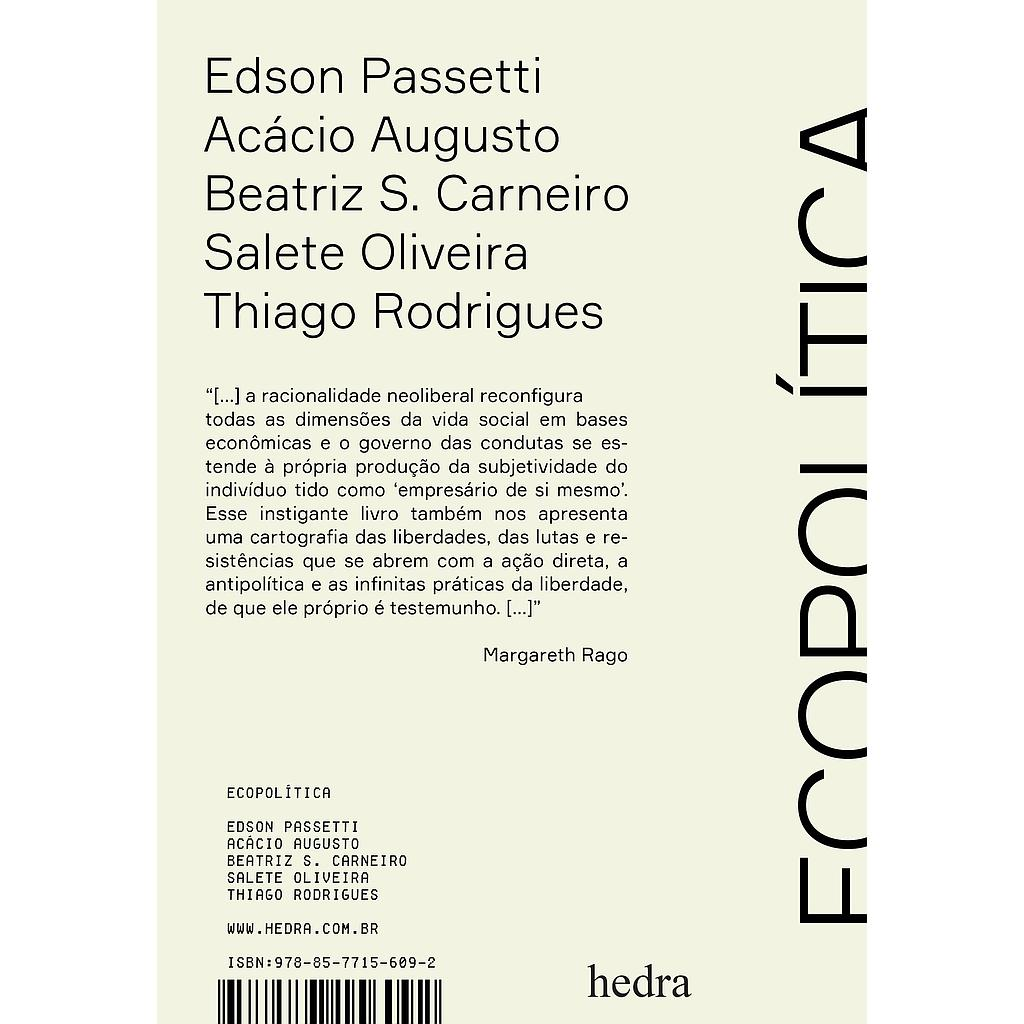
\includegraphics[width=70mm]{eco.jpeg}
%%\hspace*{6cm}\raisebox{2cm}{\rotatebox[origin=t]{90}{\Formular{\textbf{Lançamento}}}}
%\end{center}
%
%\hspace*{-2cm}\_\_\_\_\_\_\_\_\_\_\_\_\_\_\_\_\_\_\_\_\_\_\_\_\_\_\_\_\_\_\_\_\_\_\_\_\_\_\%_\_\_\_\_\_\_\_\_\_\_\_\_\_\_\_\_\_\_\_\_\_\_\_\_\_\_\_\_\_\_\_\_\_\_\_
%
%\medskip
%
%\noindent{}Lorem ipsum dolor sit amet, consectetur adipiscing elit.
%Donec sodales tortor a purus accumsan, ut ultricies purus
%maximus. Aliquam bibendum consequat mi, sed commo-
%do velit pellentesque id. Vivamus ultricies ligula in semper
%sagittis. Donec mollis odio in lectus tristique, sed convallis
%est interdum. Cras eget sem condimentum, pretium purus
%eu, auctor.
%
%\hspace{.5cm}
%
%\hspace*{-.4cm}\begin{minipage}[c]{0.45\linewidth}
%\small{
%{\Formular{\textbf{
%\hspace*{-.1cm}Título: Ecopolítica\\
%Autor: Edson Passetti\\ 
%Editora: Hedra\\
%Páginas: 476\\
%Formato: 23x16cm\\
%Preço: R\$ 79,90\\
%}}}}
%\end{minipage}
%\begin{minipage}[c]{0.50\linewidth}
%\small{Lorem ipsum dolor sit amet, consectetur adipiscing elit. Donec sodales tortor a purus accumsan, ut ultricies. Lorem ipsum dolor sit amet, %consectetur adipiscing elit. Lorem ipsum dolor sit amet. Lorem ipsum dolor sit amet.} 
%\end{minipage}
%
%\pagebreak